\documentclass[]{article}
\usepackage[T1]{fontenc}
\usepackage{lmodern}
\usepackage{amssymb,amsmath}
\usepackage{fullpage}
\usepackage{todonotes}
\usepackage{ifxetex,ifluatex}
\usepackage{fixltx2e} % provides \textsubscript
% use microtype if available
\IfFileExists{microtype.sty}{\usepackage{microtype}}{}
\ifnum 0\ifxetex 1\fi\ifluatex 1\fi=0 % if pdftex
  \usepackage[utf8]{inputenc}
\else % if luatex or xelatex
  \usepackage{fontspec}
  \ifxetex
    \usepackage{xltxtra,xunicode}
  \fi
  \defaultfontfeatures{Mapping=tex-text,Scale=MatchLowercase}
  \newcommand{\euro}{€}
\fi
% Redefine labelwidth for lists; otherwise, the enumerate package will cause
% markers to extend beyond the left margin.
\makeatletter\AtBeginDocument{%
  \renewcommand{\@listi}
    {\setlength{\labelwidth}{4em}}
}\makeatother
\usepackage{enumerate}
\usepackage{graphicx}
% We will generate all images so they have a width \maxwidth. This means
% that they will get their normal width if they fit onto the page, but
% are scaled down if they would overflow the margins.
\makeatletter
\def\maxwidth{\ifdim\Gin@nat@width>\linewidth\linewidth
\else\Gin@nat@width\fi}
\makeatother
\let\Oldincludegraphics\includegraphics
\renewcommand{\includegraphics}[1]{\Oldincludegraphics[width=\maxwidth]{#1}}
\ifxetex
  \usepackage[setpagesize=false, % page size defined by xetex
              unicode=false, % unicode breaks when used with xetex
              xetex]{hyperref}
\else
  \usepackage[unicode=true]{hyperref}
\fi
\hypersetup{breaklinks=true,
            bookmarks=true,
            pdfauthor={Harshal Pandya and Brian Martin},
            pdftitle={CS677: Lab 1},
            colorlinks=true,
            urlcolor=blue,
            linkcolor=magenta,
            pdfborder={0 0 0}}
\setlength{\parindent}{0pt}
\setlength{\parskip}{6pt plus 2pt minus 1pt}
\setlength{\emergencystretch}{3em}  % prevent overfull lines
\setcounter{secnumdepth}{0}

\title{CS677: Lab 3}
\author{Brian Martin and Harshal Pandya}
\date{}

\begin{document}
\maketitle

Our system implements the provided spec: a pig2pig network in which pigs
collaborate to avoid impact with an adversarial bird. The pigs dynamically
elect a two leaders amongst themselves and use Lamport's clocks for
synchronization. Most importantly, each leader has a local cache of pig
statuses which is consistent with the second leader's view. This is done via
with a commit protocol via an intermediate, persistent database actor. The
system also automatically fails-over when a leader fails, not losing any pig
statuses.

\subsection{Actors}
We use the actor concurrency model to enable communication between machines. The
Actor model is a mathematical model of concurrent computation that
treats ``actors'' as the universal primitives of concurrent digital
computation: in response to a message that it receives, an actor can
make local decisions, create more actors, send more messages, and
determine how to respond to the next message received. Each actor is multi-threaded 
and can send/receive messages concurrently. Moreover, we can specify whether we want 
synchronous or asynchronous semantics.

\subsection{Leader Election}
We use the ring based leader election algorithm to enable the pigs to choose a leader dynamically.
Each pig gets a random 8-digit Id at start up and the pigs organize in a logical ring in an arbitrary order.
The network topology is completely connected which allows the pigs to reorganize into a new ring in the
event one of the nodes fails. Any pig can start the election. A message is circulated along the ring and every 
pig attaches its Id to the message and passes it on. When the initiator receives the message it, it picks the 
pig with the highest Id that is alive, informs everyone about the new leader. We use a timeout to figure whether 
a pig is down and move on if the pig does not respond within a particular interval.

\subsection{Clock Synchronization}
We use Lamport's clocks to order events across the pigs. When the leader initiates the game by sending the BirdApproaching 
message it sends along its current time to all pigs. The pigs use this value to update their clocks setting it to the max of remote 
and local clock. We simulate the network latency by incrementing the clock randomly (to a value up to 5) before processing the
bird approaching message. If the pig is able to move, the clock is advanced and the time is stored as Move Time. \\
After the time to target as specified by the bird has expired the leader sends a BirdLanded message to all pigs again with its time stamp. 
The pigs simulate the network delay and after comparing the time stamp, save it as Hit Time.\\
When the leader queries the pigs for their status, they respond by comparing these clock values to decide if they were able to move before the bird hit. 
Obviously, all this happens only if the pig is impacted by the bird's landing.  

\subsection{Cache Consistency}

Cache consistency is ensured for pig statuses by a protocol which has several steps and is run on each leader:

\begin{enumerate}[1.]
    \item
        The leader makes a call to all minion pigs for their statuses.
    \item
        Status responses are collected in a buffer, which is sent to the database.
    \item
        The database blocks all other updates until the update has been passed to and commited on the other leader.
    \item
        The database reponses to the leader, waiting for acknowledgement that the original leader has commited the changes to its cache.
\end{enumerate}

This protocol is shown in Figure~\ref{commit}. There the dotted line represents
blocking. The red dots represent commits of the updates. 

Because the database is blocking during this operation, no two transactions can
overlap. This ensures strong consistency as both leaders see the same order of
events. 

This would be more important if there were ever any conflicting updates, but is
a good property to have nonetheless.

\begin{figure}
    \centering
    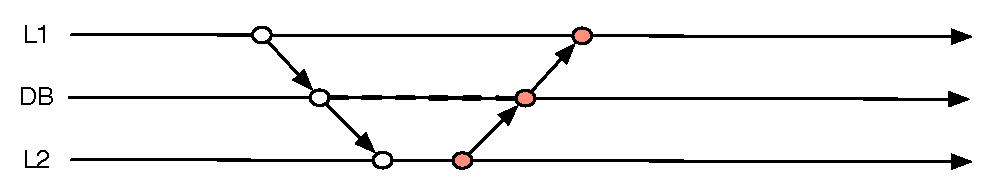
\includegraphics{figs/commit.pdf}
    \caption{The commit protocol ensuring consistnt caches between leaders.\label{commit}}
\end{figure}

\subsection{Fault Tolerance}

% This doesn't compile for some reason...
%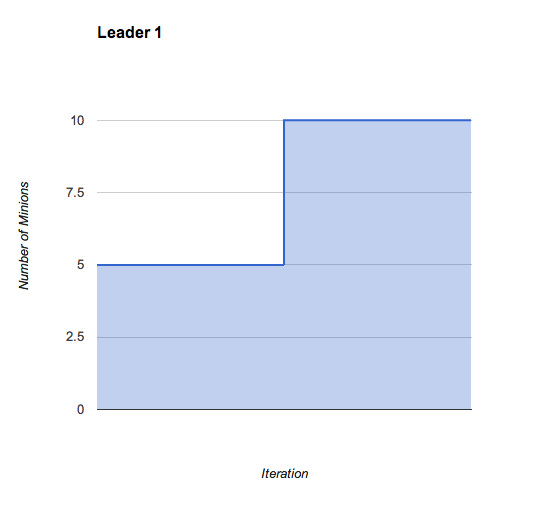
\includegraphics[height=2.7cm]{figs/num_minions.png}


It may be the case that a leader may fall asleep. In this scenario it is
necessary that the pigs which communicate with that leader move to the awake
leader. To support this it is necessary that each leader check if the other is
awake at the beginning of each iteration. If one of the leaders has fallen
asleep then the awake leader communicates which each of the orphaned pigs
telling them that he is their new leader.

In this scenario the database commit semantics must also be revised.  This is
because a full commit requires that the other leader has commited the update.
To fix this issue, we simply have the databse check if the other leader is
sleeping before asking it to commit an update. If it is asleep then the
transaction succeeds because we can not possibly block on a sleeping pig which
is blocking the transaction.

\subsection{Game Map}

The game map is single-dimensional with pigs and columns placed
randomly. It is assumed that the bird is always launched from the left
(as in the original Angry Birds). The ratio of columns to pigs is at
most one.

\subsection{Assumed Physics}

We assume that certain behaviors for each element type:

\begin{itemize}
\item
  \textbf{Pig}: An impacted pig will fall to the right (as the bird
  always approaches from the left). If a pig falls onto another pig both
  are considered impacted, but the second pig does not change position
  on impact. If a pig is impacted while having a column to the right,
  then that column will also fall to the right, affecting any pig which
  may find itself in that position.
\item
  \textbf{Column}: If a column is impacted directly, then it falls to
  the right, only affecting any pig or column to its immediate right.
\end{itemize}

\subsection{Game Engine}

In our system the \emph{game engine} has several roles:

\begin{enumerate}[1.]
\item
  Map generation
\item
  Sending round-initiating trajectory message to the leader.
\item
  Querying the leader for the status of pigs. 
\end{enumerate}

\subsection{Pigs as Actors}

Each pig functions as an actor which can receive and act on several
message types, derived from the original specification. Some of them are listed below,
please refer to the doc provided for exhaustive list.

\begin{itemize}
\item
  \texttt{Trajectory(position: Int, birdLandingTime: Clock)} notifies the leader about the birds trajectory. That is, an estimate of the bird landing time as a (future) Lamport clock value.
\item
  \texttt{BirdApproaching(targetPosition: Int, timestamp: Clock)} This message provides is used by the leader to notify the other pigs of when the bird is expected to hit. Each pig attempts to move appropriately.
\item
  \texttt{Status()} Sent by the leader to query each pig about its safety after the bird landing. Each pig determines its own safety by comparing the Lamport clock value when that pig moved to the clock value for when the bird hit.
\item
  \texttt{Election()} Any pig can send this message to any other pig (including itself) to initiate a new election.
\end{itemize}

\subsection{Launching a bird}

A bird launch is described by the time the master picks a random target
and notifies the nearest pig about the trajectory. It then picks a
random time to target before sending an end game message thus signaling
that the bird has landed.

\section{Design Decisions / Trade-offs}

The pigs form a completely connected netowork topology and so hopcounts are not
required. However, this increases the complexity of the network and it may not
scale well for larger number of nodes.The pigs don't maintain any state apart
from their current locations in the world.

We choose ring based election algorithm since it involves no synchronization
issues and is fairly robust to failures. However we make a simplifying
assumption that a pig never goes down within a round. If this was not the case
we would need to back up the state of the leader and have it communicate to
each pig after every event so that it is up to date with the state of every
pig.

Lamport's clocks are convenient for this problem since they have much less
overhead than vector clocks. Since we are only comparing local timestamps and
the messages from the leader are broadcast, we can prove the correctness of the
partial ordering we care about.

We do not maintain a shared map data structure and hence the map is not updated
when the pigs move. This however saves the effort of maintaing a synchronous
thread-safe data structure that lives on the master and adds extra messages to
the system.

\section{Possible Improvements}

We could experiment with allowing the pigs to fail while a round is being played. 
In terms of the game logic, we could use a 2
dimensional world. Also we could make pigs move make space for pigs
being affected and have the effect of hits cascade beyond 2 positions.

\section{How to run the program}

We require \texttt{sbt}, the Scala Build Tool, to compile and run the code.

Our program can be run with:

\begin{enumerate}[1.]
\item
  \textbf{\texttt{./sbt11 numPigs worldSizeRatio}}: where numPigs is the number of pigs in the simulation and worldSizeRatio is the ratio of world:pigs. For example, to run with 10 pigs on a world of size 30 you would run: ./sbt11 10 3.
\end{enumerate}

\section{Experiments:}
\missingfigure{Experiment having to do with consistency}
\missingfigure{Experiment having to do with fault-tolerance}
%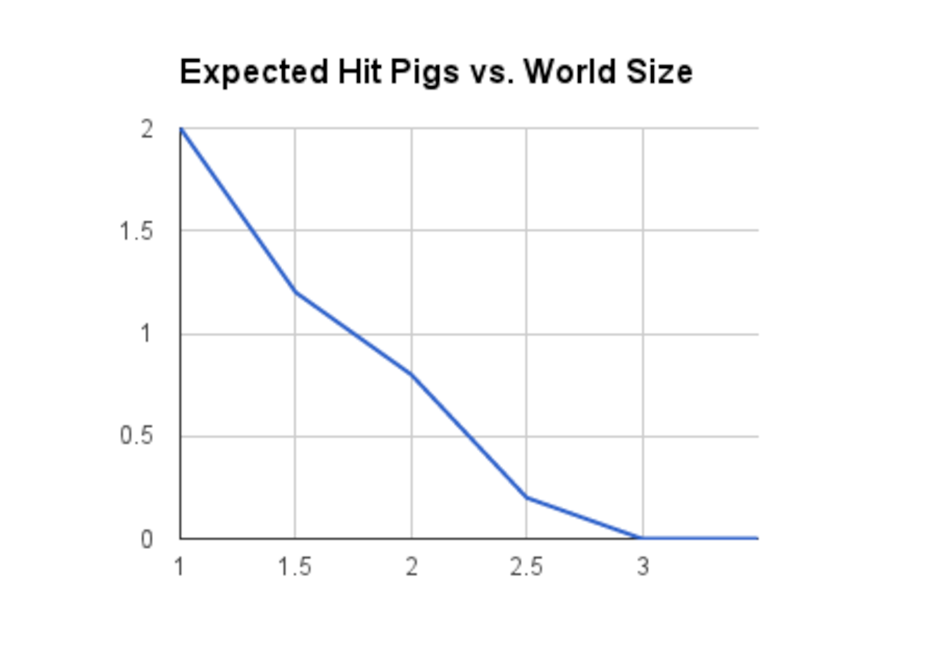
\includegraphics{figs/chart_1.pdf}
%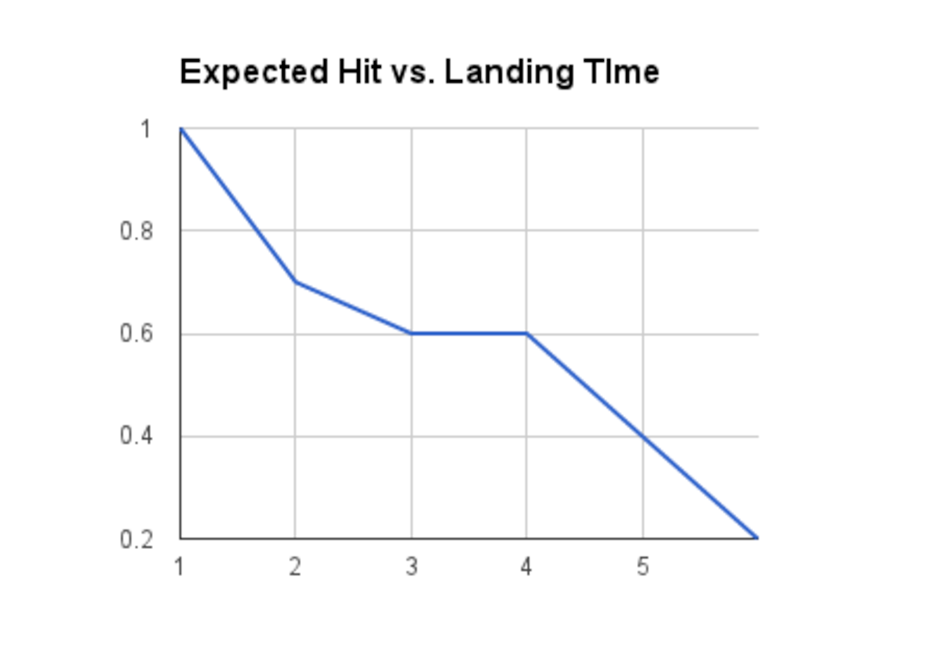
\includegraphics{figs/chart_2.pdf}

\pagebreak

\section{Test cases:}
\begin{enumerate}
\item Leader Election Test : Tests the ring based leader election algorithm by first electing a leader and then bringing a leader down to trigger reelection 
\item Cache Consistency test : Runs a round with 6 leaders and prints out the cache at the end of the round ( before database update) and after database update. Afther the update both the leaders should have the same cache.
\item Fault tolerance Test : Sends a leader to sleep and check if the responsibility of the pigs is handed off correctly to the awake leader. 
\item Dead Pig Test : Tests if the pigs dead in the previous round stay dead in subsequent rounds.
\item Game Logic Tests 1, 2 and 3: Test for different scenarios displayed in figure 
\end{enumerate}

%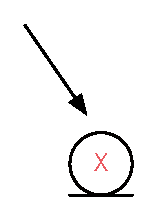
\includegraphics{figs/omni/test1.graffle} 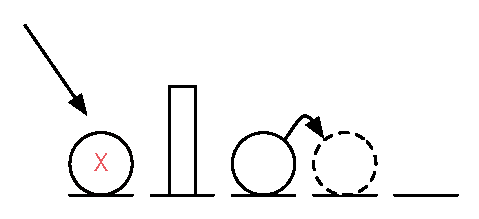
\includegraphics{figs/omni/test2.graffle}
%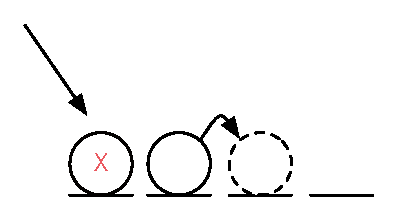
\includegraphics{figs/omni/test3.graffle} 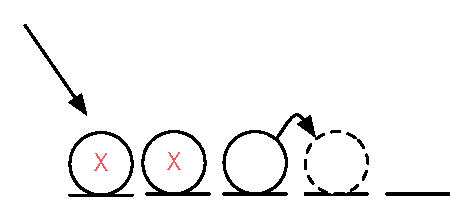
\includegraphics{figs/omni/test4.graffle}
%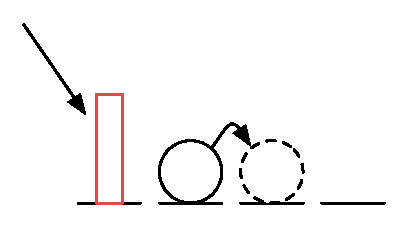
\includegraphics{figs/omni/test5.graffle}


\section{Experiments}
We did 2 major experiments:
\begin{enumerate}[1.]
\item
  Expected number of pigs hit as function of the world size to number of pigs ratio.
\item
  Expected number of pigs hit as function of the the bird landing time.
\end{enumerate} 

\section{Sample Election Output:}

The following is the log of 10 pigs being started and two elections occurring over disjoint subsets of pigs.
\tiny\begin{verbatim}
[info] DEBUG [2013-05-08 00:46:51,649] com.github.harshal.distos.PigsRunner: Ring arranger ids: 10001, 10002, 10003, 10004
[info] DEBUG [2013-05-08 00:46:51,658] com.github.harshal.distos.Pig: 10001 received neighbor list: SetNeighbors(WrappedArray(10002, 10003, 10004))
[info] DEBUG [2013-05-08 00:46:51,698] com.github.harshal.distos.Pig: 10002 received neighbor list: SetNeighbors(WrappedArray(10003, 10004, 10001))
[info] DEBUG [2013-05-08 00:46:51,709] com.github.harshal.distos.Pig: 10003 received neighbor list: SetNeighbors(WrappedArray(10004, 10001, 10002))
[info] DEBUG [2013-05-08 00:46:51,720] com.github.harshal.distos.Pig: 10004 received neighbor list: SetNeighbors(WrappedArray(10001, 10002, 10003))
[info] DEBUG [2013-05-08 00:46:51,731] com.github.harshal.distos.PigsRunner: Ring arranger ids: 10005, 10006, 10007, 10008
[info] DEBUG [2013-05-08 00:46:51,732] com.github.harshal.distos.Pig: 10005 received neighbor list: SetNeighbors(WrappedArray(10006, 10007, 10008))
[info] DEBUG [2013-05-08 00:46:51,744] com.github.harshal.distos.Pig: 10006 received neighbor list: SetNeighbors(WrappedArray(10007, 10008, 10005))
[info] DEBUG [2013-05-08 00:46:51,754] com.github.harshal.distos.Pig: 10007 received neighbor list: SetNeighbors(WrappedArray(10008, 10005, 10006))
[info] DEBUG [2013-05-08 00:46:51,764] com.github.harshal.distos.Pig: 10008 received neighbor list: SetNeighbors(WrappedArray(10005, 10006, 10007))
[info] DEBUG [2013-05-08 00:46:51,775] com.github.harshal.distos.PigsRunner: Sending DebugNeighbors..
[info] DEBUG [2013-05-08 00:46:51,776] com.github.harshal.distos.PigsRunner: Initiating an election in set 1..
[info] INFO  [2013-05-08 00:46:51,778] com.github.harshal.distos.Pig: 10008 Neighbors: 46539603,3fbf1e64,dfc68a75
[info] INFO  [2013-05-08 00:46:51,778] com.github.harshal.distos.Pig: 10003 Neighbors: f711b65b,947cf6b5,d4f82124
[info] INFO  [2013-05-08 00:46:51,778] com.github.harshal.distos.Pig: 10005 Neighbors: 3fbf1e64,dfc68a75,2d88ed78
[info] INFO  [2013-05-08 00:46:51,778] com.github.harshal.distos.Pig: 10001 Neighbors: d4f82124,0691b452,f711b65b
[info] INFO  [2013-05-08 00:46:51,778] com.github.harshal.distos.Pig: 10007 Neighbors: 2d88ed78,46539603,3fbf1e64
[info] INFO  [2013-05-08 00:46:51,778] com.github.harshal.distos.Pig: 10002 Neighbors: 0691b452,f711b65b,947cf6b5
[info] DEBUG [2013-05-08 00:46:51,778] com.github.harshal.distos.PigsRunner: Initiating an election in set 2..
[info] INFO  [2013-05-08 00:46:51,778] com.github.harshal.distos.Pig: 10006 Neighbors: dfc68a75,2d88ed78,46539603
[info] INFO  [2013-05-08 00:46:51,778] com.github.harshal.distos.Pig: 10004 Neighbors: 947cf6b5,d4f82124,0691b452
[info] DEBUG [2013-05-08 00:46:51,796] com.github.harshal.distos.Pig: Election from 947cf6b5 -> d4f82124, succeeded...
[info] DEBUG [2013-05-08 00:46:51,796] com.github.harshal.distos.Pig: Election from 46539603 -> 3fbf1e64, succeeded...
[info] DEBUG [2013-05-08 00:46:51,797] com.github.harshal.distos.Pig: Election from d4f82124 -> 0691b452, succeeded...
[info] DEBUG [2013-05-08 00:46:51,797] com.github.harshal.distos.Pig: Election from 3fbf1e64 -> dfc68a75, succeeded...
[info] DEBUG [2013-05-08 00:46:51,799] com.github.harshal.distos.Pig: Election from dfc68a75 -> 2d88ed78, succeeded...
[info] DEBUG [2013-05-08 00:46:51,800] com.github.harshal.distos.Pig: Election from 0691b452 -> f711b65b, succeeded...
[info] INFO  [2013-05-08 00:46:51,800] com.github.harshal.distos.Pig: Election 8d3f0588 finished: dfc68a75 is the leader.
[info] INFO  [2013-05-08 00:46:51,800] com.github.harshal.distos.Pig: Election aa40338e finished: f711b65b is the leader.
[info] DEBUG [2013-05-08 00:46:51,803] com.github.harshal.distos.Pig: Election from 2d88ed78 -> 46539603, succeeded...
[info] DEBUG [2013-05-08 00:46:51,803] com.github.harshal.distos.Pig: Election from f711b65b -> 947cf6b5, succeeded...
[info] DEBUG [2013-05-08 00:46:51,806] com.github.harshal.distos.Pig: 3fbf1e64 setting leader to dfc68a75
[info] DEBUG [2013-05-08 00:46:51,806] com.github.harshal.distos.Pig: d4f82124 setting leader to f711b65b
[info] DEBUG [2013-05-08 00:46:51,809] com.github.harshal.distos.Pig: 0691b452 setting leader to f711b65b
[info] DEBUG [2013-05-08 00:46:51,809] com.github.harshal.distos.Pig: dfc68a75 setting leader to dfc68a75
[info] DEBUG [2013-05-08 00:46:51,809] com.github.harshal.distos.Pig: 10007 initiating db connection.
[info] DEBUG [2013-05-08 00:46:51,813] com.github.harshal.distos.Pig: f711b65b setting leader to f711b65b
[info] DEBUG [2013-05-08 00:46:51,813] com.github.harshal.distos.Pig: 10004 initiating db connection.
[info] DEBUG [2013-05-08 00:46:51,817] com.github.harshal.distos.DB: Added 10007 as leader.
[info] DEBUG [2013-05-08 00:46:51,818] com.github.harshal.distos.DB: Added 10004 as leader.
[info] DEBUG [2013-05-08 00:46:51,821] com.github.harshal.distos.Pig: 947cf6b5 setting leader to f711b65b
[info] DEBUG [2013-05-08 00:46:51,822] com.github.harshal.distos.Pig: 2d88ed78 setting leader to dfc68a75
[info] DEBUG [2013-05-08 00:46:51,830] com.github.harshal.distos.Pig: 46539603 setting leader to dfc68a75
[info] DEBUG [2013-05-08 00:46:53,286] com.github.harshal.distos.Pig: Leader (10004) set secondary leader to: 10007
[info] DEBUG [2013-05-08 00:46:53,287] com.github.harshal.distos.Pig: Leader (10007) set secondary leader to: 10004
[info] INFO  [2013-05-08 00:46:53,289] com.github.harshal.distos.PigsRunner: generating the map..
[info] DEBUG [2013-05-08 00:46:53,305] com.github.harshal.distos.Pig: Secondary leader is awake. 10007 continuing as normal.
[info] DEBUG [2013-05-08 00:46:53,305] com.github.harshal.distos.Pig: Secondary leader is awake. 10004 continuing as normal.
[info] DEBUG [2013-05-08 00:46:53,305] com.github.harshal.distos.Pig: 10004: Ack'ing CheckIfAwake.
[info] DEBUG [2013-05-08 00:46:53,305] com.github.harshal.distos.Pig: 10007: Ack'ing CheckIfAwake.
\end{verbatim}


\normalsize

\end{document}
